\documentclass[11pt]{article}

\usepackage{amsmath}
\usepackage{textcomp}
\usepackage[top=0.8in, bottom=0.8in, left=0.8in, right=0.8in]{geometry}
\usepackage{listings}
\usepackage{graphicx}
\usepackage{subcaption}
\usepackage[linesnumbered,lined,boxed,commentsnumbered]{algorithm2e}
\SetKwRepeat{Do}{do}{while}%

% add other packages here

% put your group number and names in the author field
\title{\bf Exercise 2: A Reactive Agent for the Pickup and Delivery Problem}
\author{Group 24: Benvenuti Eloi Jean, Timoth\'ee-Florian S\'ebastien Bronner}

% the report should not be longer than 3 pages

\begin{document}
\maketitle

\section{Problem Representation}

\subsection{Representation Description}
% describe how you design the state representation, the possible actions, the reward table and the probability transition table
\paragraph{State representation} A state is defined by the city in which the vehicle is, whether there is an available task in the city and, if there is, to which city the task requires the vehicle to move to. Since the agent will be presented only one task even if there are multiple available tasks in the city, there is no need to add extra states for the cases where they are some combinations of available tasks in the city.

This means that, for each city, there is (n-1), where n is the number of cities, state where a task is available (one for each other city) and 1 state for when no task is available. Since there are n cities, this gives us a total of $\text{n}^2$ states.

\paragraph{Possible actions} When he is in a city the vehicle can either pick up the available task and go to the corresponding city, if a task is available, or not pick up anything and move to a neighboring city.

\paragraph{Reward table} In order to decide on the best action we need to know, for each state, the best expected rewards. We store those in a dictionary with an entry for each state.

\paragraph{Probability transition table} By picking our actions we can control in which city we end up. The random part is the state of the city (whether there will be a task and to which city the task require us to go). We didn't need to construct this table because we could query all the probabilities by an API call.

\subsection{Implementation Details}
% describe the implementation details of the representations above and the implementation details of the reinforcement learning algorithm you implemented
\paragraph{State class} The state class has 3 variables:
\begin{itemize}
  \item startCity: The city in which the vehicle currently is.  
  \item endCity: The city in which the task requires us to go. This is equal to null if there is no available task.
  \item task: A boolean who is equal to true if there is a task in the city, and false otherwise.
\end{itemize}

\paragraph{AgentMove class} The AgentMove class encodes the different actions the vehicle can take. It has 3 variables:
\begin{itemize}
  \item startCity: The city in which the vehicle currently is.
  \item endCity: The city in which the vehicle will move.
  \item task: A boolean who is equal to true if the vehicle do this movement in the context of picking up and delivering a task and false otherwise.
\end{itemize}

\paragraph{Reward HashTable} We encoded the best reward for each state into a \lstinline{HashMap<State,Double>} who takes states as key and returns the expected rewards.

\paragraph{Best action HashTable} We encoded the best action for each state into a \lstinline{HashMap<State,AgentMove>} who takes states as key and returns the best move encoded in the AgentMove class.

\paragraph{Iterative computation of the reward table} We computed the best actions and optimal rewards following this procedure:



\begin{algorithm}[H]
 \SetAlgoLined
 \KwData{States $s\in S$, actions $a \in A$, forgetting factor $\gamma$, probability transition table $T$}
 \KwResult{Best expected reward for each state V, best action for each state}

 Initialize V=0 and V\_=0 for all states\;
 \Do{$|V(s) - V\_(s)| < \epsilon \quad \forall s \in S$}{
 V\_ = V \;
 \For{$s \in S$}{
  \For{$a \in A$}
   {
   $R(s,a) = \text{expected rewards of the task} - \text{cost of movement}$ \;
   $Q(s,a) = R(s,a) + \gamma \sum_{s' \in S} T(s,a,s') * V\_(s')$ \;
   }
   $a_{max} = \text{find\_max}(Q(s,a \quad \forall a \in A))$ \;
   $V(s) = Q(s,a_{max})$ \;
   $\text{bestAction}(s) = a_{max}$ \;
  }
 }
 \caption{Computation of the best action and the best expected reward.}
\end{algorithm}

\section{Results}
% in this section, you describe several results from the experiments with your reactive agent

  
\subsection{Experiment 1: Discount factor}
% the purpose of this experiment is to understand how the discount factor influences the result
This experiment aims at providing an understanding of the influence that the discount factor has over the efficiency of the agent.

\subsubsection{Setting}
% you describe how you perform the experiment (you also need to specify the configuration used for the experiment)
To analyse the role of discount factor 5 measurements of the average reward ( reward per step) for each discount factor have been averaged. The measurements have been made at 6000 steps. This average is shown in Figure \ref{fig:discount factors}, note that most measurements are made with discount factors close to 1. 

\subsubsection{Observations}
% you describe the experimental results and the conclusions you inferred from these results
The result shown in Figure \ref{fig:discount factors} indicates that at low discount factors will be prejudicial to the efficiency of the agent. However, after 0.75 a plateau can be observed and increasing the discount factor does not improve the result. It should also be noted that changing the discount factor could only improve the efficiency by a couple of percentage (3.1\% between the two maxima). This seems to indicate that the algorithm implemented is only marginally improving compared to the greedy algorithm (discount factor of 0).
\begin{figure}
  \centering
  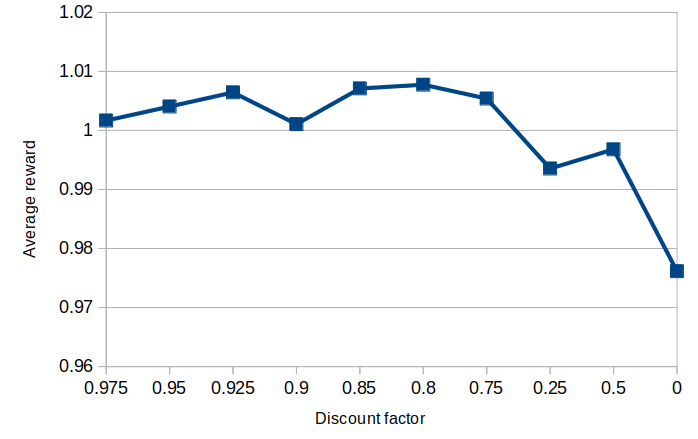
\includegraphics[width=0.5\textwidth]{experiment/df.png}
  \caption{\label{fig:discount factors} Normalized average reward per step}
\end{figure}

\subsection{Experiment 2: Comparisons with dummy agents}
% you compare the results of your agent with two dummy agents: the random agent that was already given in the starter files and another dummy agent that you define and create. You should report the results from the simulations using the topologies given in the starter files and optionally, additional topologies that you create.
The reactive agent will now be compared to two dummy agents.
\subsubsection{Setting}
% you describe how you perform the experiment and you describe the dummy agent you created (you also need to specify the configuration used for the experiment)
The comparison will be made between the worst case of the reactive agent in function of the discount factor (0) and two dummy classifiers. To see if the worst case is still more efficient. 
The two dummies are implemented as follows:
\begin{enumerate}
  \item If a task is available randomly chose to pick it up. If no task taken randomly move to a connected city.
  \item If there is no task randomly move to a connected city, otherwise pick the task.
\end{enumerate}

\subsubsection{Observations}
% elaborate on the observed results
The results are again made by averaging 5 average reward (reward per step). The result is the following.
\begin{itemize}
  \item Worst reactive: 37844
  \item Dummy 1 (pure random): 31212
  \item Dummy 2 (always pick up an available task): 36135

\end{itemize}

This shows that the reactive agents perform, even in the worst case, better that the dummy agents. Even though the simple fact that an agent who will always take an available task can make it relatively close (4.5 \% of difference) to our greedy agent. 


\end{document}
